\section{Introduction}

Understanding the past climate of the earth allows for us to begin to understand what effects we are having upon it, and to predict what the future will bring.
From ice cores, a rough temperature record of Earth is constructed and we explain attempt to explain that.
The variation in the orbital parameters of our planet affect the amount of solar insolation recieved, and the timescale variation of these quantities is one possible forcing for past climatic change.
The eliptical elements of the orbit are changing slowly in time, as is the orientation of the planet's spin axis.
A three state model from Paillard fits the data emprically, and we attempt a rigorous fit of this model to data using the tools of evolutionary computation.

\section{Paillard's Model}

With some difficulty understanding his original paper \cite{paillard1998timing}, we recontruct Paillard's model for both versions that he provides.
The following two subsections paraphrase \cite{paillard1998timing} directly.

\subsection{Discrete model}

\newcommand{\inter}{\textbf{i}}
\newcommand{\mild}{\textbf{g}}
\newcommand{\full}{\textbf{G}}

The model has three states called \inter~(interglacial), \mild~(mild glacial) and \full~(full glacial).
This model undergoes an \inter-\mild~transistion as soon as the insolation falls below $i_0$.
An \mild-\full~transistion happens when the ice volume exceeds a threshold $v_\text{max}$ and finally a transistion \full-\inter~occurs when the insolation increases above $i_1$.
These transistions are assumed to be one-way, and the only ones allowed are those just discussed.
The \mild-\full~transition has the constraints that it will happen after some time $t_g$ and with insolation lower than some level $i_3$.
If $t_g$ is exceeded but $i_3$ is also exceeded, then the \mild-\full~transistion occurs as the next insolation decrease: when insolation falls below $i_2$.
% THIS MODEL IS WEIRDDDDDD

The part which was made least clear was whether the insolation exceeding $i_3$ necessitates a reset of the time in state \mild until $t_g$ is reached.
To achieve similar results, we assume that the answer is yes, the time does reset.



\subsection{Differential equation model}

This model is an extension of the discrete model.
There are still three regimes but now we define the ice volume $v$ as a differential equation

$$ \frac{dv}{dt} = (v_R - v) /\tau _R - F/\tau _F .$$

where $R$ is the current climate regime ($R$ = \inter,\mild,\full), $v_R$ are the reference ice volumes for the different regimes, $F$ is the forcing and $\tau _{R,F}$ are the time constants.
The transistions are the same for \inter-\mild~and \full-\mild~but \mild-\full~now happens when $v \geq v_\text{max}$, some threshold value (without any condition on the insolation).
Paillard also ``normalizes the ice volume to unity'': $v_g = v_G = v_\text{max} = 1$ and $v_i = 0$.
For the finale of model weirdness, the forcing $F$ is defined as a truncated insolation signal with truncation function $f$ as

$$ f(x) = \frac{1}{2} \left ( x + \sqrt{4a^2 + x^2} \right ) $$

and setting $a=1$.

\section{Computing Insolation}

The only input to the model is the solar insolation, so we are particulary careful to obtain accurate values.
Increasingly accurate integrations of the state of the solar system have been performed dating from the time of Lagrange in 1781 through Milankovich's use of Pilgrim's 1904 computations to establish his theory of past climate change to today's direct numerical integrations \cite{laskar2004long}.

Using the orbital parameters of eccentricity $e$, obliquity $\epsilon$, and longitude of the parahelion $\overline{\omega}$ computed from an integration function insola.f provided from Laskar \cite{laskar2004long} we can reconstruct the insolation at any time.
The following derivation is due to Berger \cite{berger1981long}.

The insolation $Q$ at a given location and time can be written as a function of the solar constant $S_0$, the distance from the Earth to sun relative to the average $R_0/R_E$ the solar zenith angle $\Theta$:

$$ Q = S_0 \frac{R_0^2}{R_E^2} \cos (\Theta) .$$

To solve for the average insolation during one day at a given latitute $\phi$, we need to express the solar zenith angle $\Theta$ in terms of $\phi$ and the known orbital parameters.
Taking $\delta$ as the latitude of the point directly subsolar and $h$ as the hour angle, we use the spherical law of cosines to write

$$ \cos ( \Theta ) = \sin ( \phi ) \sin ( \delta ) + \cos ( \phi ) \cos ( \delta ) \cos ( h ) .$$

Now to have the average daily insolation $\overline{Q} _\text{day}$ we take the integral of $Q$ from $h_o $ to $-h_0$ where $h_0$ is the hour angle for which the sun first rises.
Since we are concerned with the $\phi = $65N, the sun always rises and sets so we won't consider the cases for the sun neither rising nor setting.
Integrating, we have

$$ \overline{Q} _\text{day} = \frac{S_0}{\pi } \frac{R_0^2}{R_E^2} \left [ h_0 \sin (\phi) \sin (\delta) + \cos (\phi) \cos (\delta) \sin (h_0) \right ] . $$

Defining $\theta = 0$ the be the vernal equinox, we can write $\delta$ and $R_0/R_E$ as a function of the orbital parameters in a simple form at the summer solsctice ($\theta = \pi /2$):

$$ \delta = \epsilon ~~~~\text{and} ~~~~ \frac{R_0}{R_E} = 1 + e\sin (\overline {\omega}) .$$

\section{Evolutionary Algorithm Methods}



Morgan

\section{Results}

Figure \ref{fig:insol-data} depicts the reconstruction of insolation data back in time.

\begin{figure}[tpb!]
\centering
  \includegraphics[width=.48\textwidth]{../data/insolation/insol_data2_noname.pdf}
  \caption{
    The average daily solar insolation $\overline{Q}_{\text{day}}$ is computed on the summer solstice at 65N with the prodived $e,\epsilon,$ and $\overline{\omega}$.
  }
  \label{fig:insol-data}
\end{figure}

Figure \ref{fig:paillard-fig3} is a direct representation of the second figure of Paillard's original paper \cite{paillard1998timing}.

\begin{figure}[tpb!]
\centering
  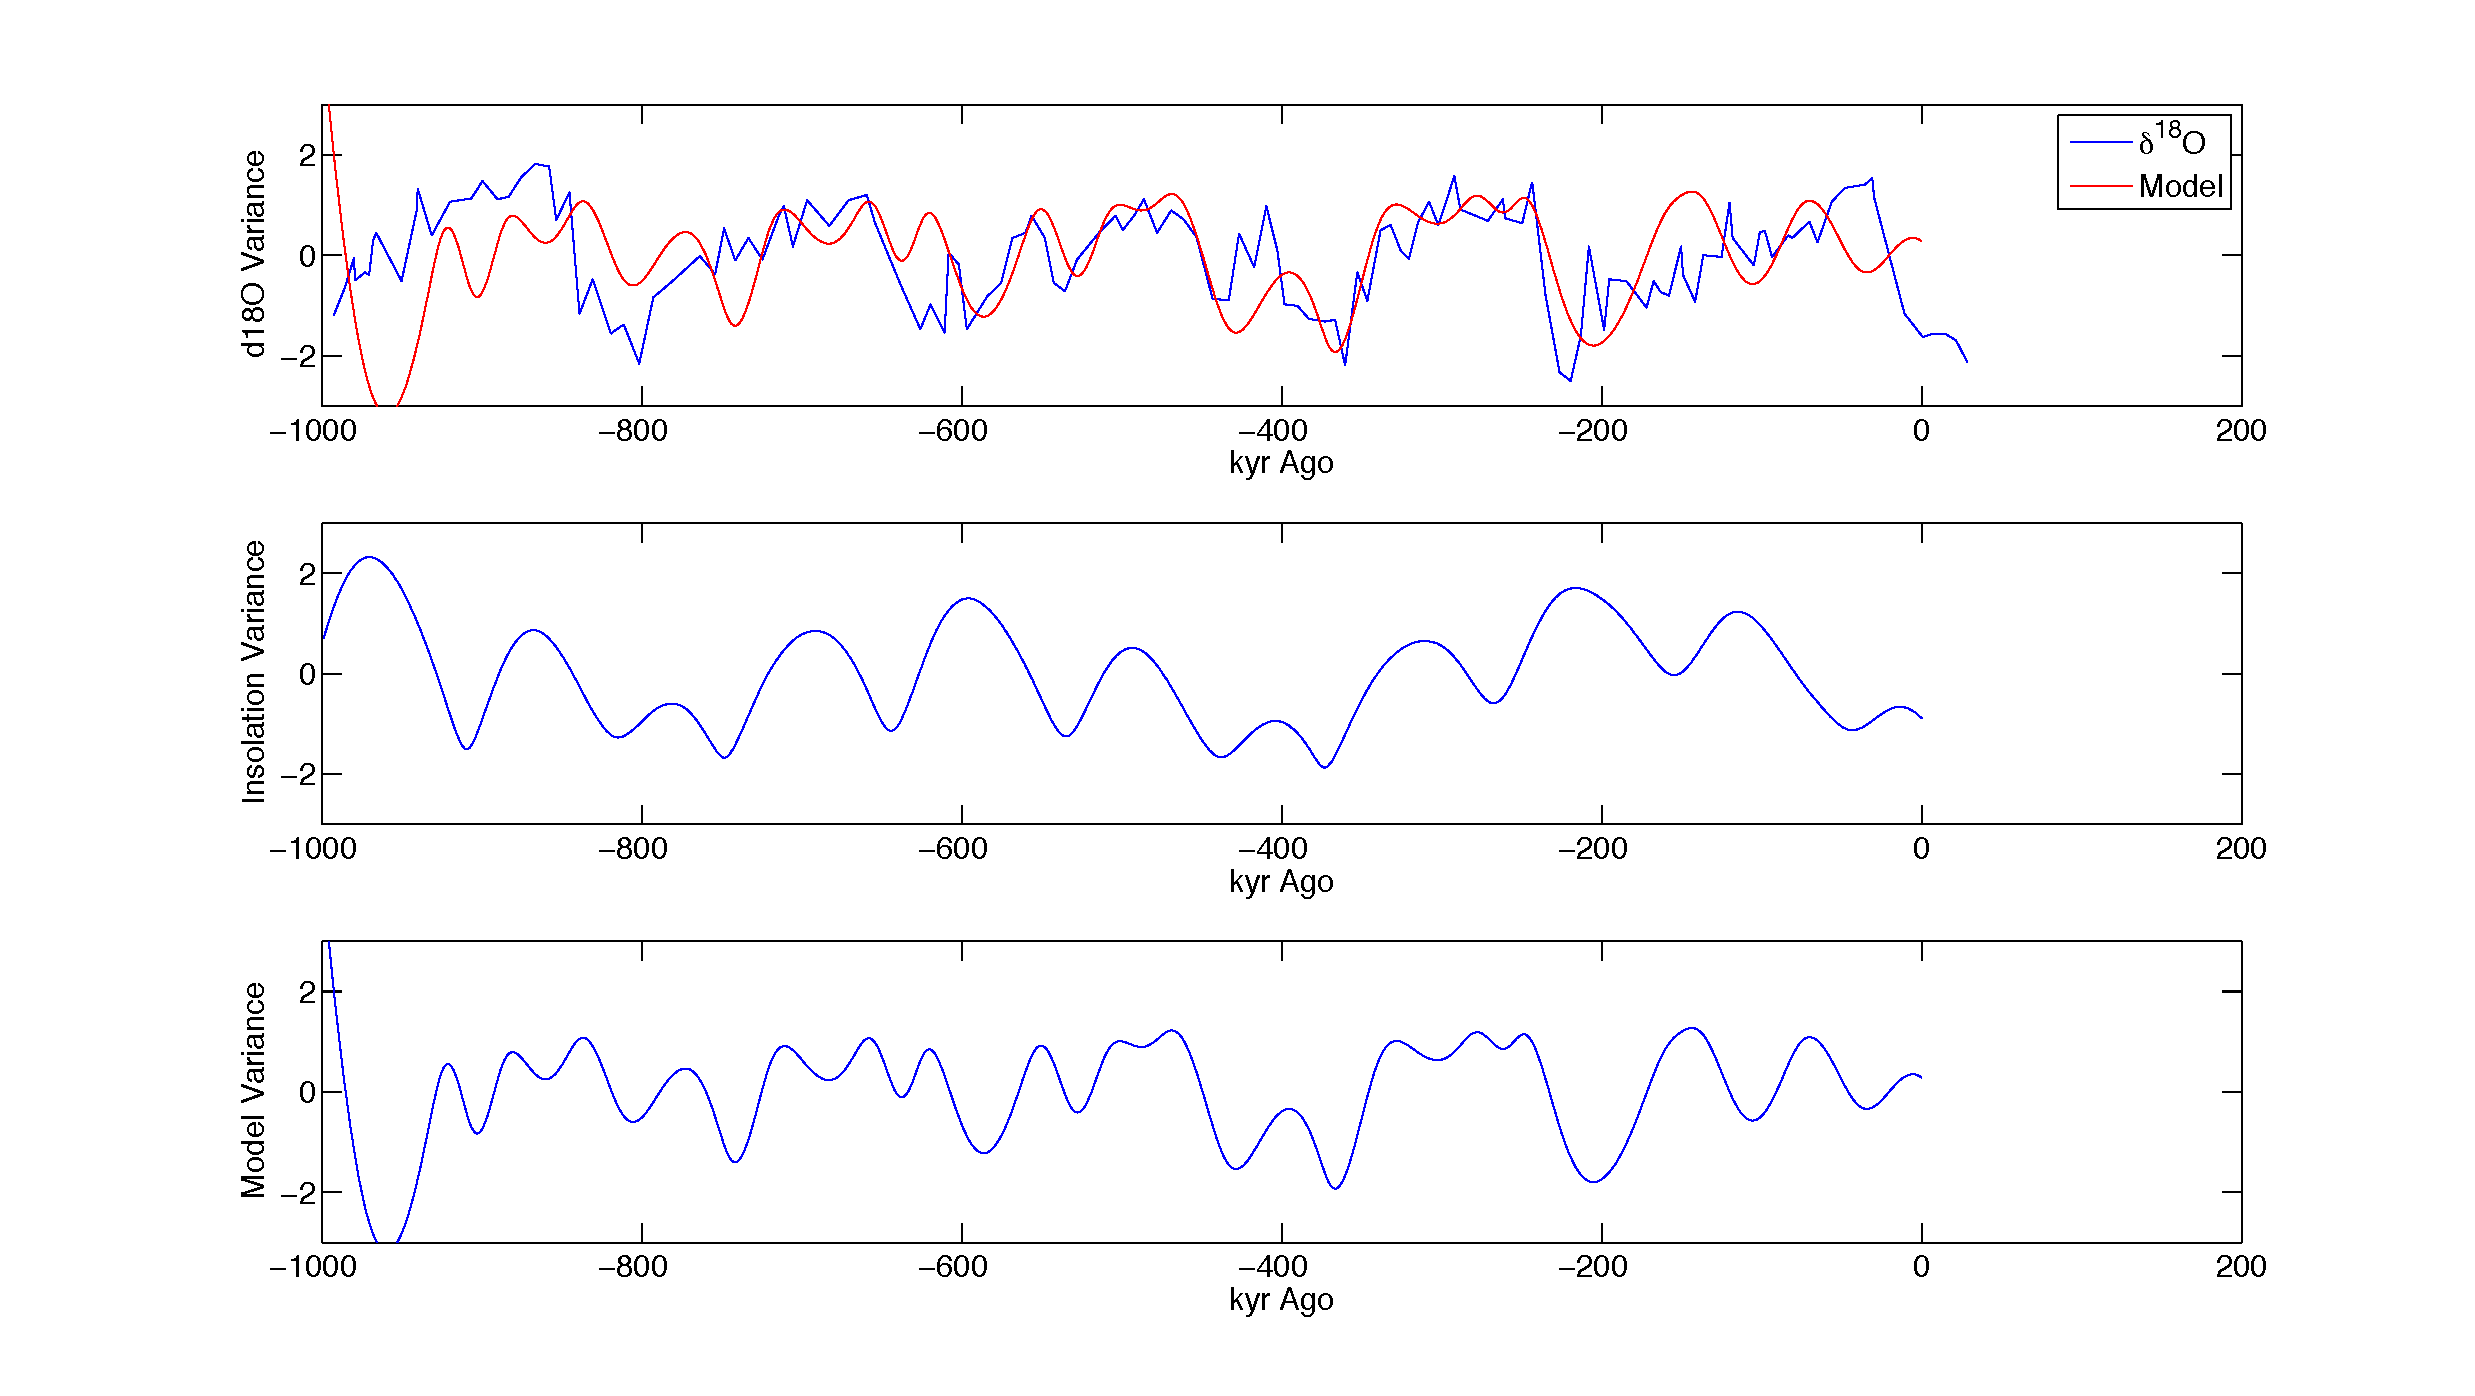
\includegraphics[width=.53\textwidth]{paillardFig3.pdf}
  \caption{
    A first run of the Paillard ODE model, over the $\delta ^{18} O$ record show a reasonable emprical fit.
  }
  \label{fig:paillard-fig3}
\end{figure}

\begin{figure}[tpb!]
\centering
  \includegraphics[width=.45\textwidth]{../src/discrete_plot_noname.pdf}
  \caption{
    The discrete Paillard model.
  }
  \label{fig:paillard-fig3}
\end{figure}


\section{Conclusion}

The fitted Paillard-Reagan-Frank model of climatic variability wholly explains the temperature variation in the $\delta ^{18} O$ record.
With only forcing from changing solar insolation, this verifies that past climatic varaition of larger time scales is a result of the variation of the Earth's orbital parameters.


